\section{Color Transformations to DES Bandpasses Diagnostic Plots}
\label{app:colorplots}
\subsection{Dark Energy Survey (DES) Y6 Calibration Stars}
Since DES is the internal bandpass used for \monster all color transformations are the null transform.

\subsection{Gaia XP Synthetic Magnitudes}
% XP g
\begin{figure}
    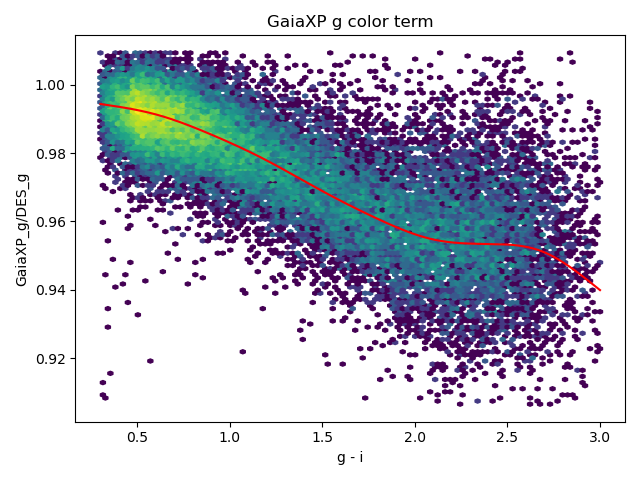
\includegraphics[width=0.49\linewidth]{./figures/color_terms/GaiaXP_to_DES_band_g_color_term.png}
    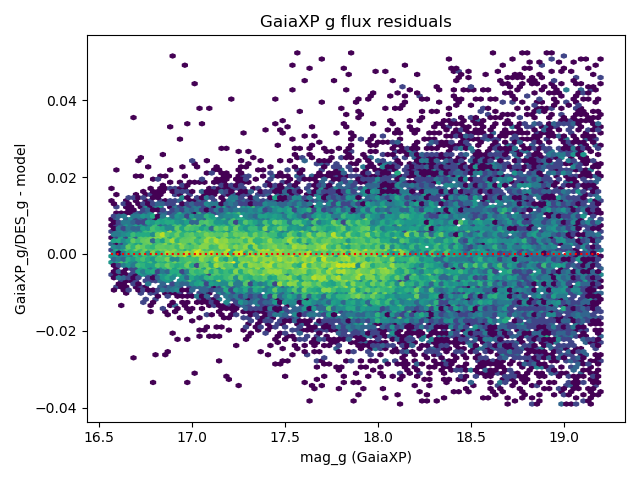
\includegraphics[width=0.49\linewidth]{./figures/color_terms/GaiaXP_to_DES_band_g_flux_residuals.png}
    \caption{Left: The ratio of fluxes between \emph{Gaia}-XP synthetic photometry and DES for the \textit{g}-band as a function of \textit{g-i} color. The red line shows the cubic spline that defines our color transformation.
    Right: Residuals between \emph{Gaia}-XP synthetic photometry transformed to DES and DES as a function of magnitude.}
    \label{fig:acolor-xp-g}
\end{figure}
% XP-DES r
\begin{figure}
    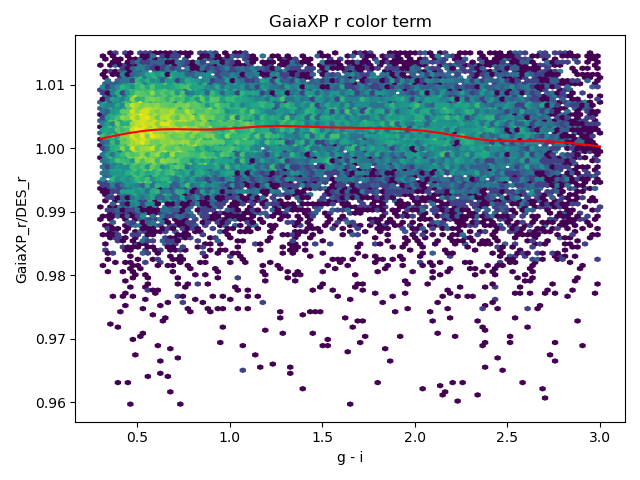
\includegraphics[width=0.49\linewidth]{./figures/color_terms/GaiaXP_to_DES_band_r_color_term.png}
    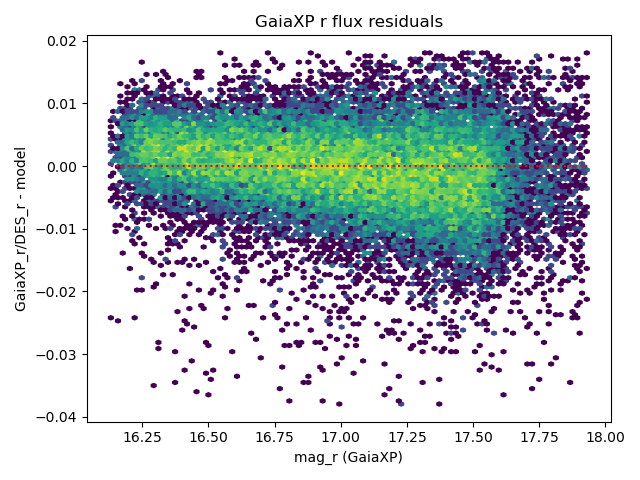
\includegraphics[width=0.49\linewidth]{./figures/color_terms/GaiaXP_to_DES_band_r_flux_residuals.png}
    \caption{Same as figure \ref{fig:acolor-xp-g} but for \textit{r}-band}
\end{figure}
% XP-DES i
\begin{figure}
    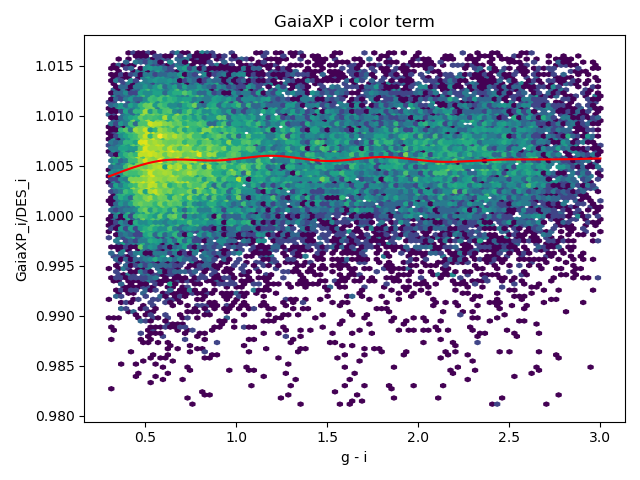
\includegraphics[width=0.49\linewidth]{./figures/color_terms/GaiaXP_to_DES_band_i_color_term.png}
    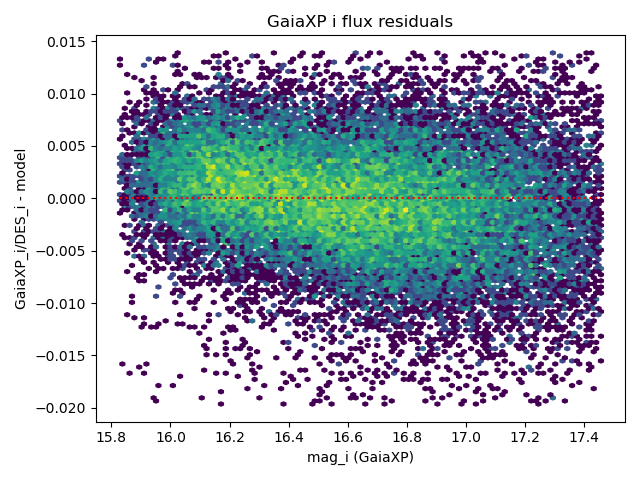
\includegraphics[width=0.49\linewidth]{./figures/color_terms/GaiaXP_to_DES_band_i_flux_residuals.png}
    \caption{Same as figure \ref{fig:acolor-xp-g} but for \textit{i}-band}
\end{figure}
% XP-DES z
\begin{figure}
    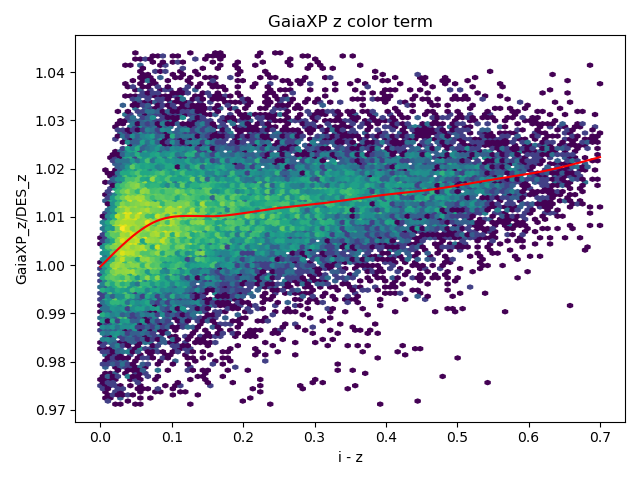
\includegraphics[width=0.49\linewidth]{./figures/color_terms/GaiaXP_to_DES_band_z_color_term.png}
    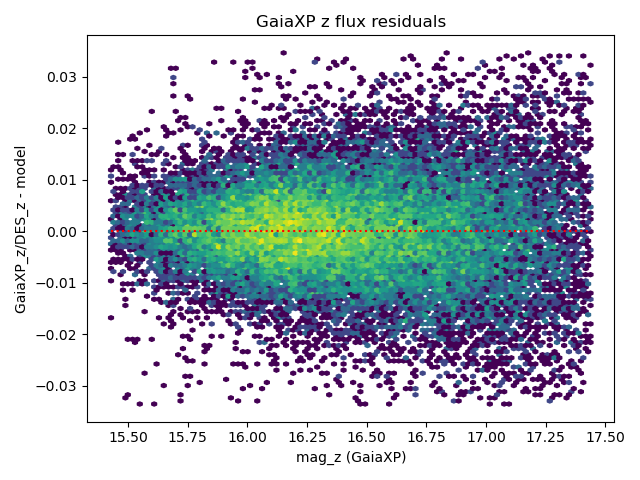
\includegraphics[width=0.49\linewidth]{./figures/color_terms/GaiaXP_to_DES_band_z_flux_residuals.png}
    \caption{Same as figure \ref{fig:acolor-xp-g} but for \textit{z}-band. Note the color transfomation is a function of i-z}
\end{figure}
% XP-DES y
\begin{figure}
    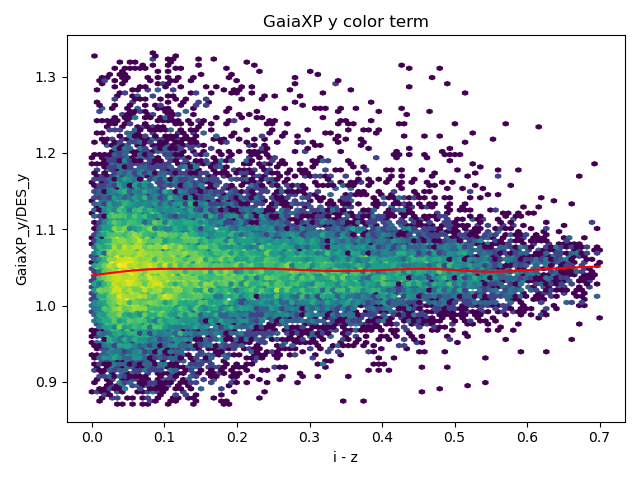
\includegraphics[width=0.49\linewidth]{./figures/color_terms/GaiaXP_to_DES_band_y_color_term.png}
    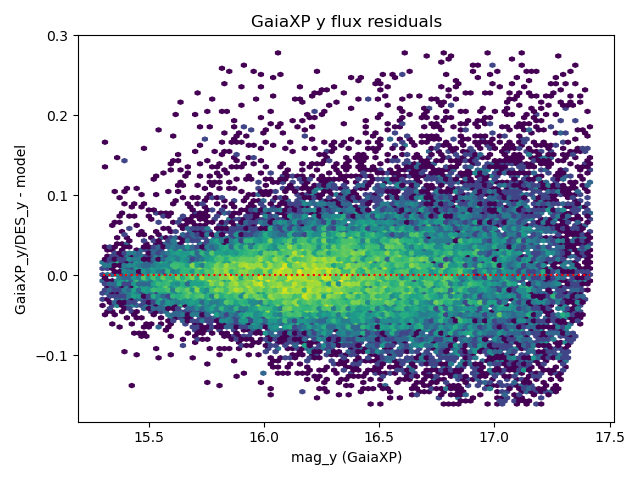
\includegraphics[width=0.49\linewidth]{./figures/color_terms/GaiaXP_to_DES_band_y_flux_residuals.png}
    \caption{Same as figure (\ref{fig:acolor-xp-g}) but for \textit{y}-band. Note the color transfomation is a function of i-z}
\end{figure}


\clearpage
\subsection{PanSTARRS1 (PS1)}
\label{sec:ps1-color}
% PS1-DES g
\begin{figure}
    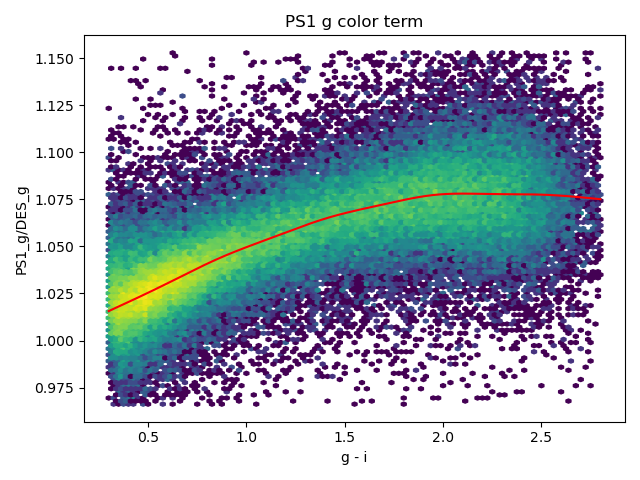
\includegraphics[width=0.49\linewidth]{./figures/color_terms/PS1_to_DES_band_g_color_term.png}
    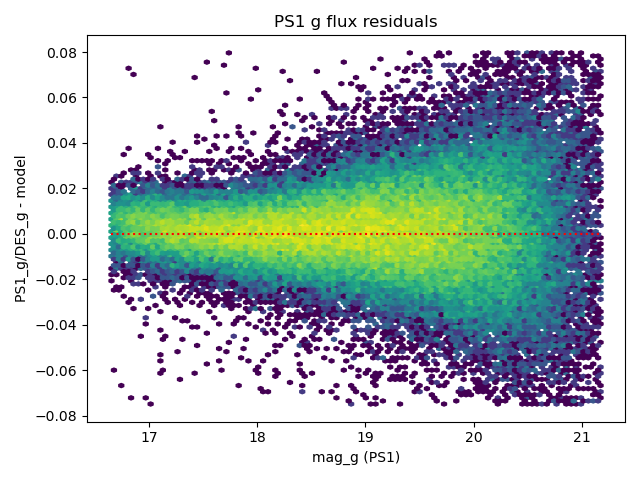
\includegraphics[width=0.49\linewidth]{./figures/color_terms/PS1_to_DES_band_g_flux_residuals.png}
    \caption{Left: The ratio of fluxes between PS1 photometry and DES for the \textit{g}-band as a function of \textit{g-i} color. The red line shows the cubic spline that defines our color transformation.
    Right: Residuals between \emph{Gaia}-XP synthetic photometry transformed to DES and DES as a function of magnitude.}
    \label{fig:acolor-ps1-g}
\end{figure}

% PS1-DES r
\begin{figure}
    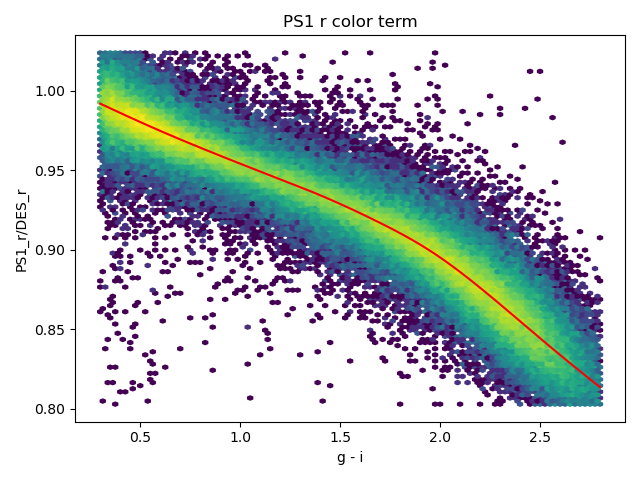
\includegraphics[width=0.49\linewidth]{./figures/color_terms/PS1_to_DES_band_r_color_term.png}
    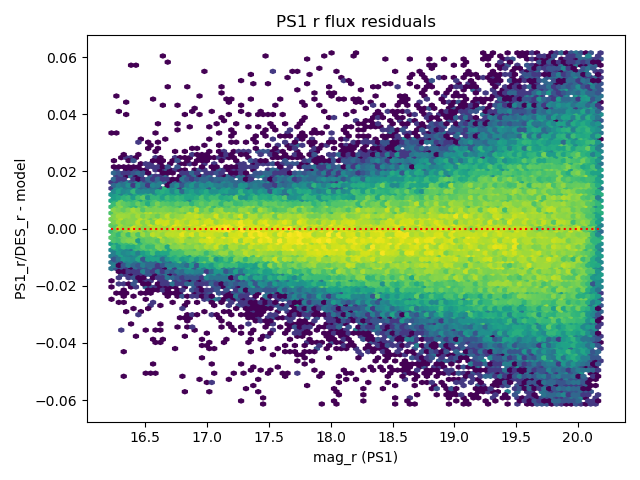
\includegraphics[width=0.49\linewidth]{./figures/color_terms/PS1_to_DES_band_r_flux_residuals.png}
    \caption{Same as figure (\ref{fig:acolor-ps1-g}) but for \textit{r}-band.}
   
\end{figure}

% PS1-DES i
\begin{figure}
    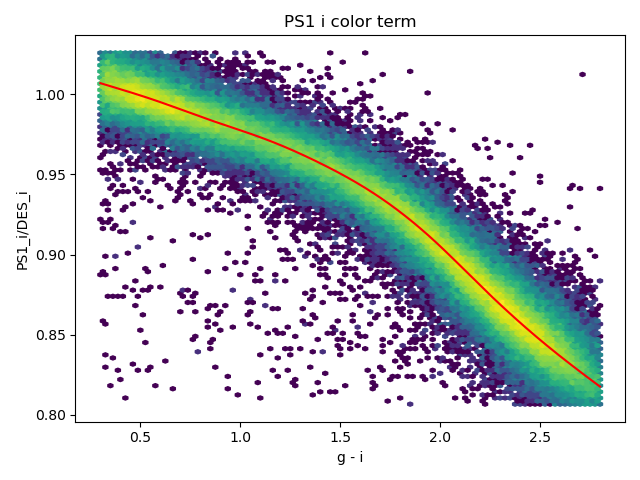
\includegraphics[width=0.49\linewidth]{./figures/color_terms/PS1_to_DES_band_i_color_term.png}
    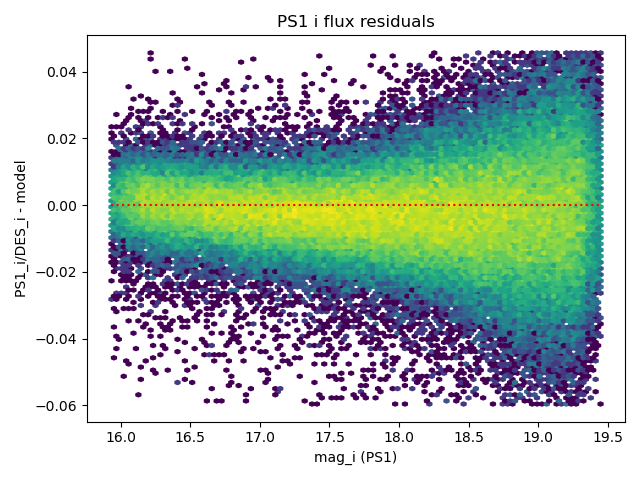
\includegraphics[width=0.49\linewidth]{./figures/color_terms/PS1_to_DES_band_i_flux_residuals.png}
    \caption{Same as figure (\ref{fig:acolor-ps1-g}) but for \textit{i}-band.}
\end{figure}
% PS1-DES z
\begin{figure}
    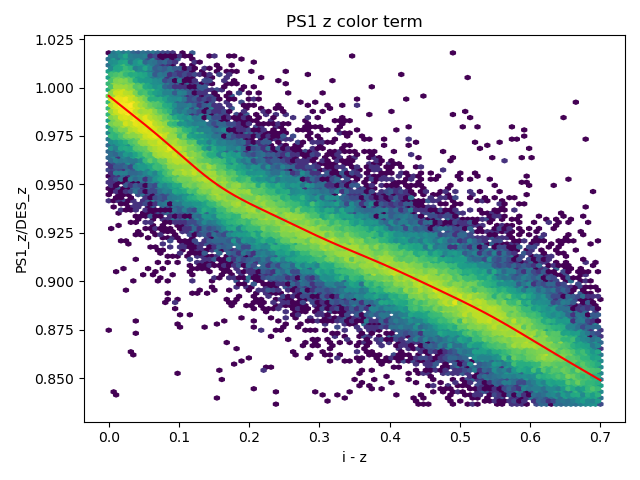
\includegraphics[width=0.49\linewidth]{./figures/color_terms/PS1_to_DES_band_z_color_term.png}
    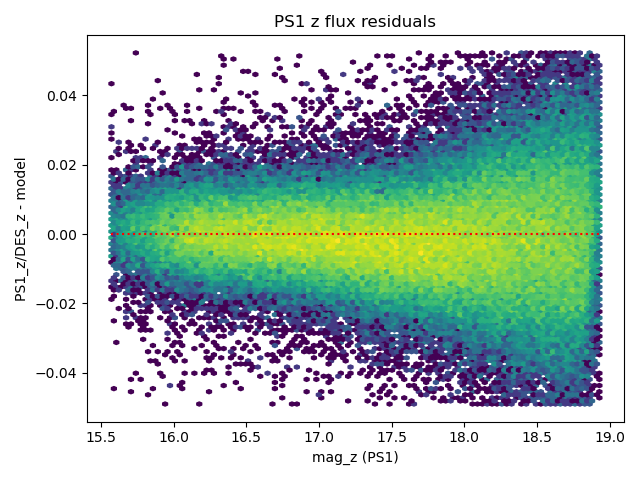
\includegraphics[width=0.49\linewidth]{./figures/color_terms/PS1_to_DES_band_z_flux_residuals.png}
    \caption{Same as figure (\ref{fig:acolor-ps1-g}) but for \textit{z}-band. Note the color transfomation is a function of i-z}
\end{figure}
% PS1-DES y
\begin{figure}
    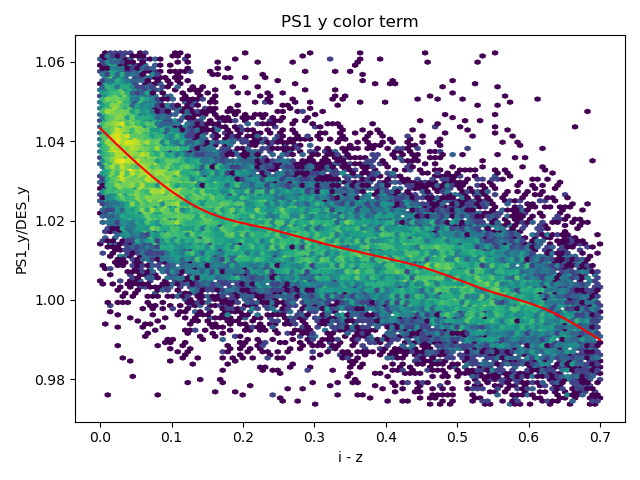
\includegraphics[width=0.49\linewidth]{./figures/color_terms/PS1_to_DES_band_y_color_term.png}
    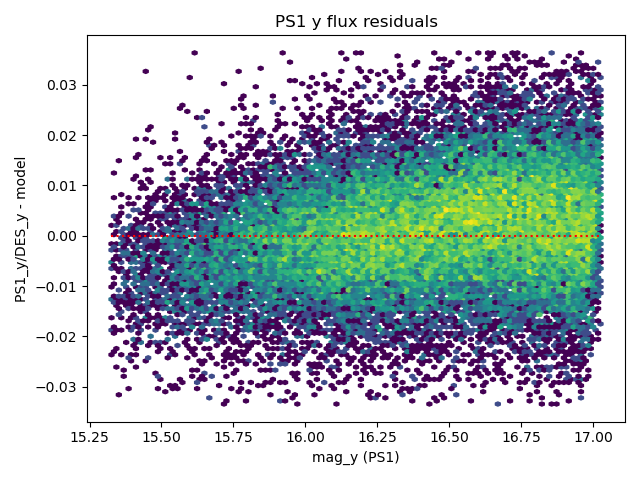
\includegraphics[width=0.49\linewidth]{./figures/color_terms/PS1_to_DES_band_y_flux_residuals.png}
    \caption{Same as figure (\ref{fig:acolor-ps1-g}) but for \textit{y}-band. Note the color transfomation is a function of i-z}
\end{figure}
For PS1 we also fit a magnitude dependent offset to bring the bright end of the PS1 photometry into agreement with the \emph{Gaia}-XP photometry, the relations are included in the color terms and shown in figure \ref{fig:mag_spline_ps1}. 
\begin{figure}
    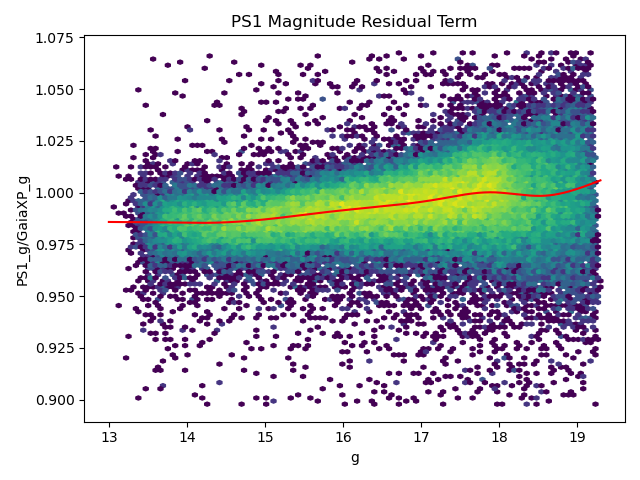
\includegraphics[width=0.49\linewidth]{./figures/color_terms/mag_offset/PS1_vs_GaiaXP_band_g_mag_offset.png}
    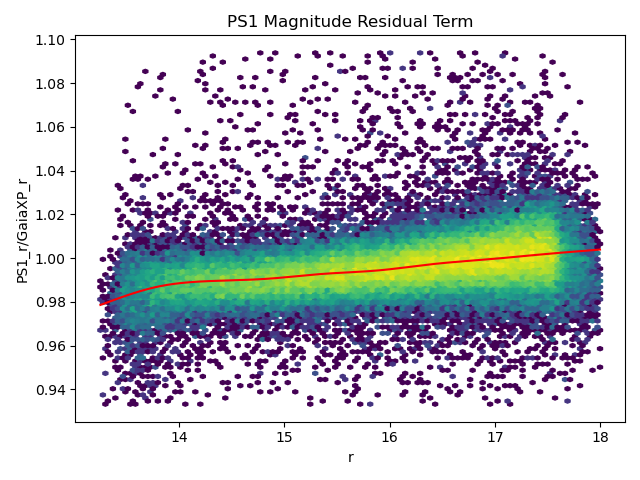
\includegraphics[width=0.49\linewidth]{./figures/color_terms/mag_offset/PS1_vs_GaiaXP_band_r_mag_offset.png}
    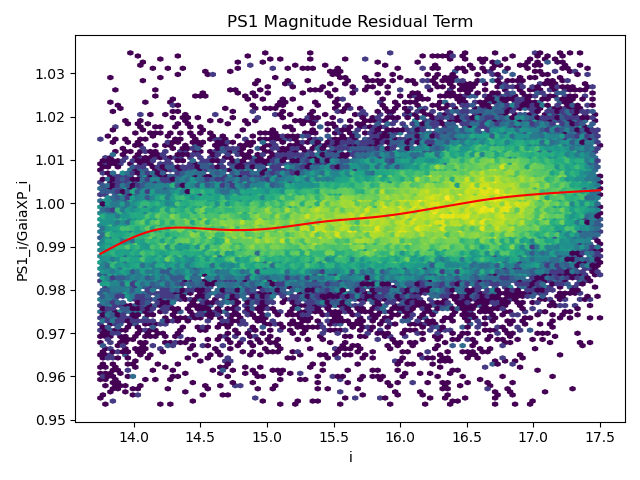
\includegraphics[width=0.49\linewidth]{./figures/color_terms/mag_offset/PS1_vs_GaiaXP_band_i_mag_offset.png}
    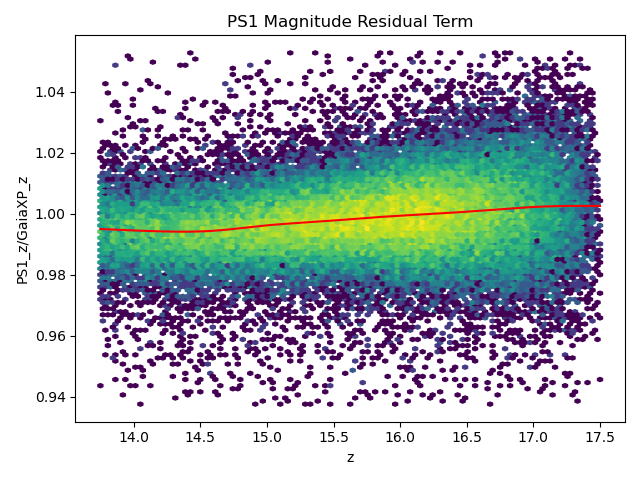
\includegraphics[width=0.49\linewidth]{./figures/color_terms/mag_offset/PS1_vs_GaiaXP_band_z_mag_offset.png}
    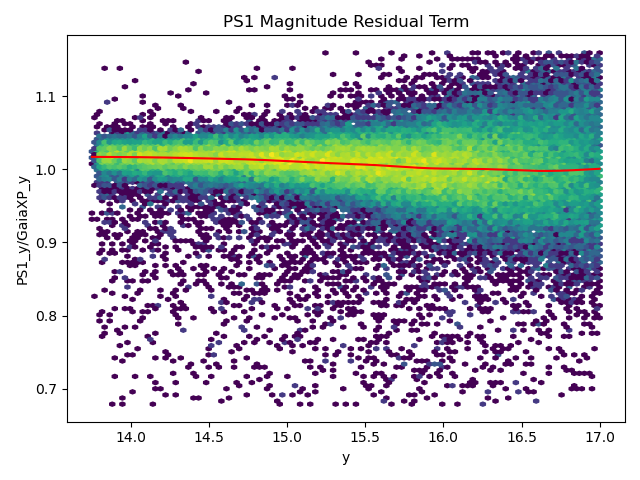
\includegraphics[width=0.49\linewidth]{./figures/color_terms/mag_offset/PS1_vs_GaiaXP_band_y_mag_offset.png}
    \caption{Magnitude dependent offsets for PS1 photometry in the DES bandpasses when compared with \emph{Gaia}-XP synthetic photometry in the DES bandpasses. The offsets are shown as a function of DES magnitude. The red line shows the cubic spline that defines our color transformation.}
    \label{fig:mag_spline_ps1}
\end{figure}
\clearpage
\subsection{SkyMapper}
% sm-DES g
\begin{figure}
    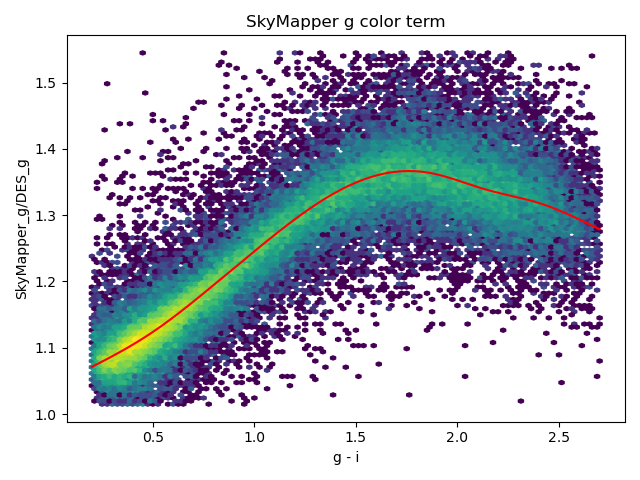
\includegraphics[width=0.49\linewidth]{./figures/color_terms/SkyMapper_to_DES_band_g_color_term.png}
    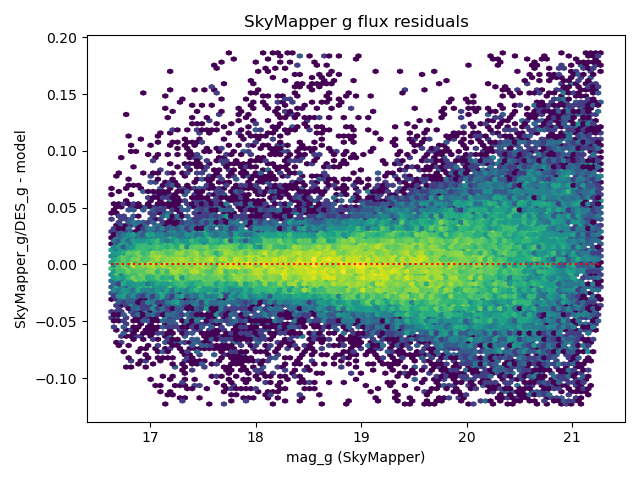
\includegraphics[width=0.49\linewidth]{./figures/color_terms/SkyMapper_to_DES_band_g_flux_residuals.png}
    \caption{Left: The ratio of fluxes between SkyMapper photometry and DES for the \textit{g}-band as a function of \textit{g-i} color. The red line shows the cubic spline that defines our color transformation.
    Right: Residuals between \emph{Gaia}-XP synthetic photometry transformed to DES and DES as a function of magnitude.}
    \label{fig:acolor-sm-g}
\end{figure}
% sm-DES r
\begin{figure}
    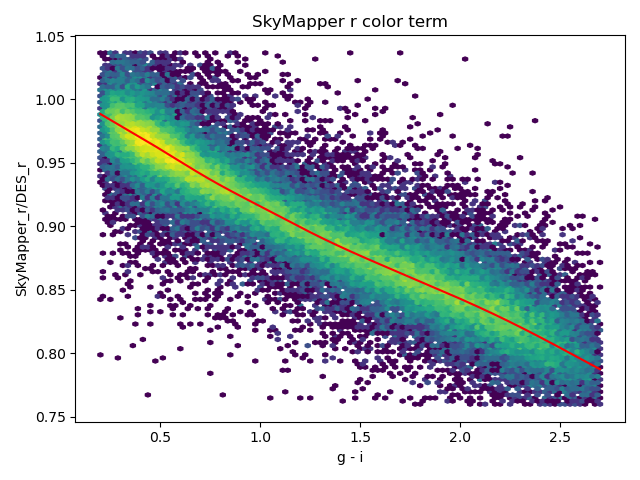
\includegraphics[width=0.49\linewidth]{./figures/color_terms/SkyMapper_to_DES_band_r_color_term.png}
    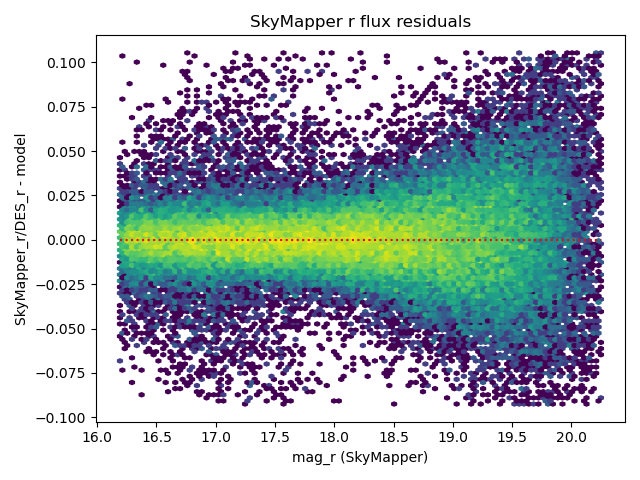
\includegraphics[width=0.49\linewidth]{./figures/color_terms/SkyMapper_to_DES_band_r_flux_residuals.png}
    \caption{Same as figure (\ref{fig:acolor-sm-g}) but for \textit{r}-band.}
\end{figure}
% sm-DES i
\begin{figure}
    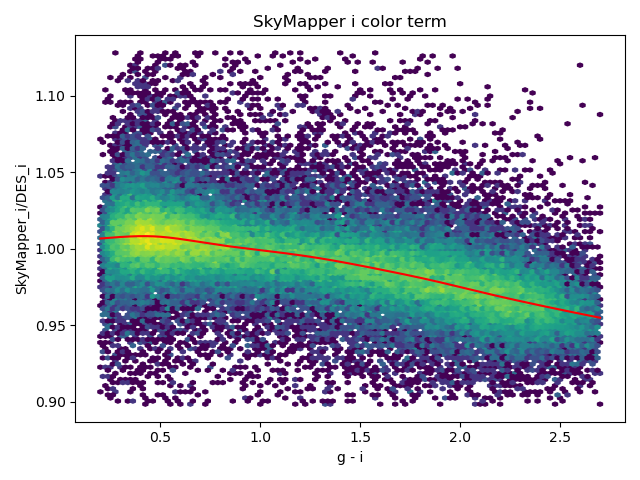
\includegraphics[width=0.49\linewidth]{./figures/color_terms/SkyMapper_to_DES_band_i_color_term.png}
    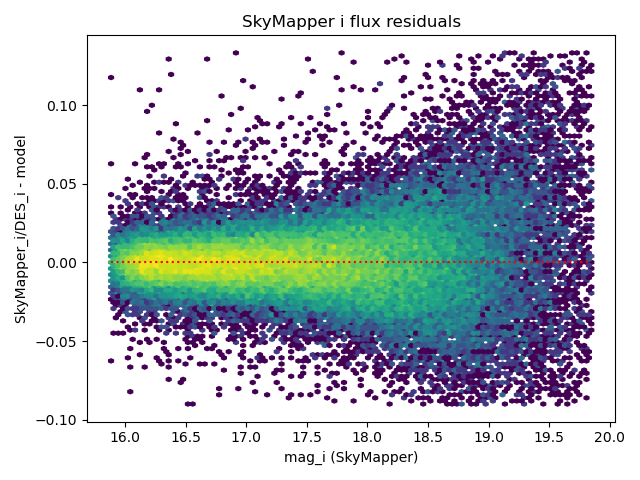
\includegraphics[width=0.49\linewidth]{./figures/color_terms/SkyMapper_to_DES_band_i_flux_residuals.png}
    \caption{Same as figure (\ref{fig:acolor-sm-g}) but for \textit{i}-band.}
\end{figure}
% sm-DES z
\begin{figure}
    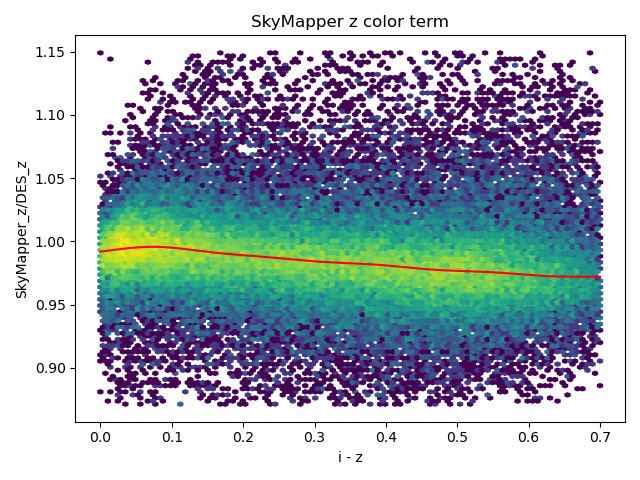
\includegraphics[width=0.49\linewidth]{./figures/color_terms/SkyMapper_to_DES_band_z_color_term.png}
    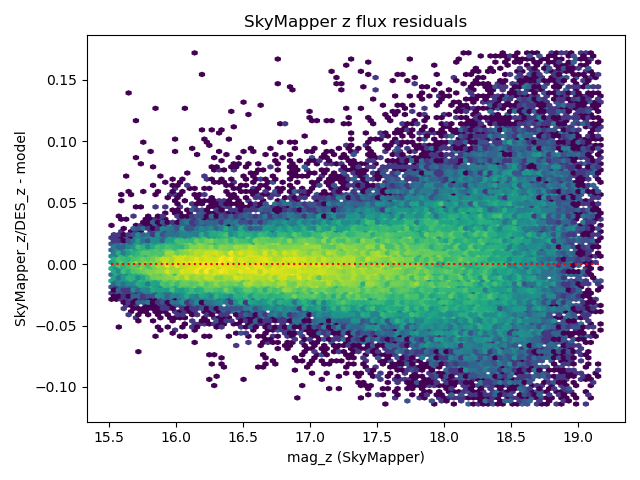
\includegraphics[width=0.49\linewidth]{./figures/color_terms/SkyMapper_to_DES_band_z_flux_residuals.png}
    \caption{Same as figure (\ref{fig:acolor-sm-g}) but for \textit{z}-band. Note the color transfomation is a function of i-z}
\end{figure}

\clearpage
\subsection{VST}
% vst-DES g
\begin{figure}
    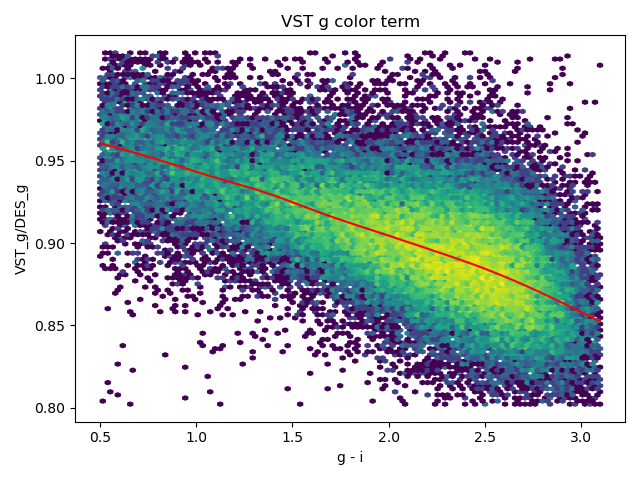
\includegraphics[width=0.49\linewidth]{./figures/color_terms/VST_to_DES_band_g_color_term.png}
    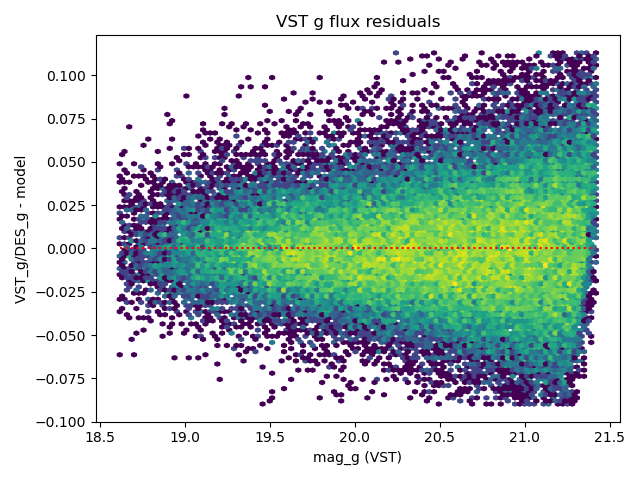
\includegraphics[width=0.49\linewidth]{./figures/color_terms/VST_to_DES_band_g_flux_residuals.png}
    \caption{Left: The ratio of fluxes between VST ATLAS photometry and DES for the \textit{g}-band as a function of \textit{g-i} color. The red line shows the cubic spline that defines our color transformation.
    Right: Residuals between \emph{Gaia}-XP synthetic photometry transformed to DES and DES as a function of magnitude.}
    \label{fig:acolor-vst-g}
\end{figure}
% vst-DES r
\begin{figure}
    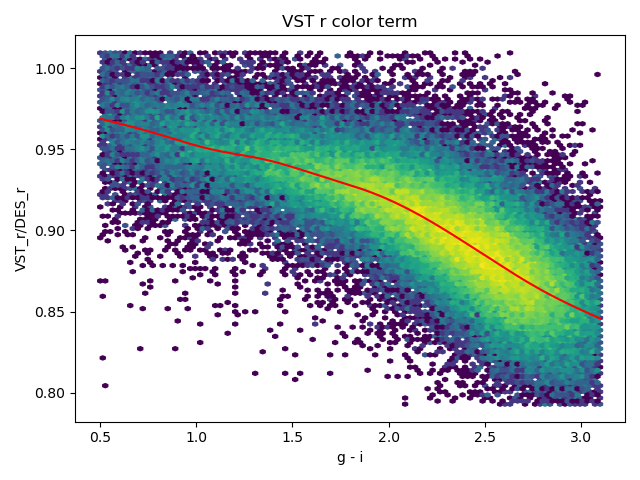
\includegraphics[width=0.49\linewidth]{./figures/color_terms/VST_to_DES_band_r_color_term.png}
    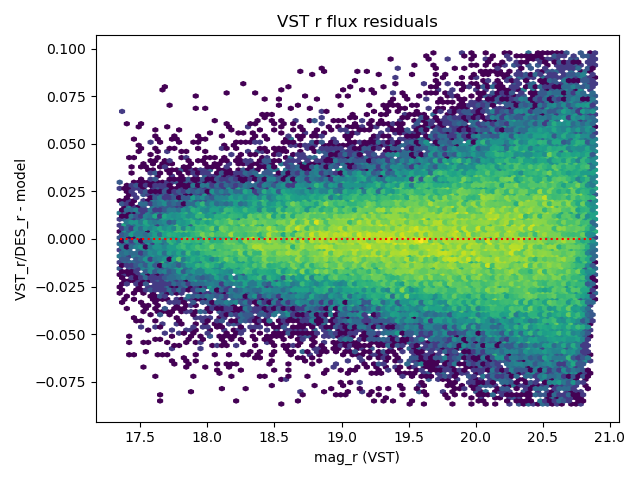
\includegraphics[width=0.49\linewidth]{./figures/color_terms/VST_to_DES_band_r_flux_residuals.png}
    \caption{Same as figure (\ref{fig:acolor-vst-g}) but for \textit{r}-band.}
\end{figure}
% vst-DES i
\begin{figure}
    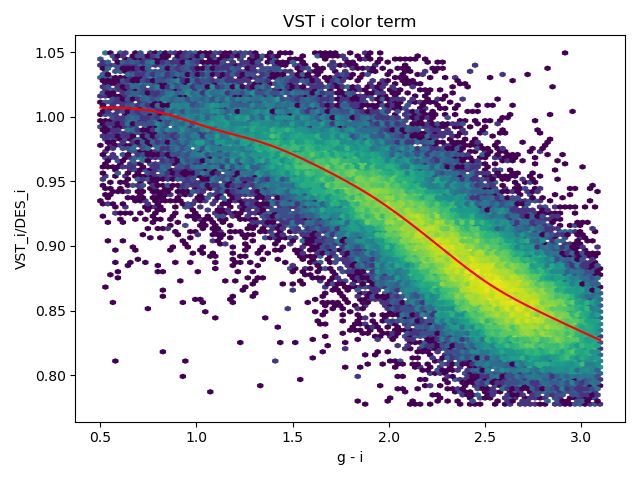
\includegraphics[width=0.49\linewidth]{./figures/color_terms/VST_to_DES_band_i_color_term.png}
    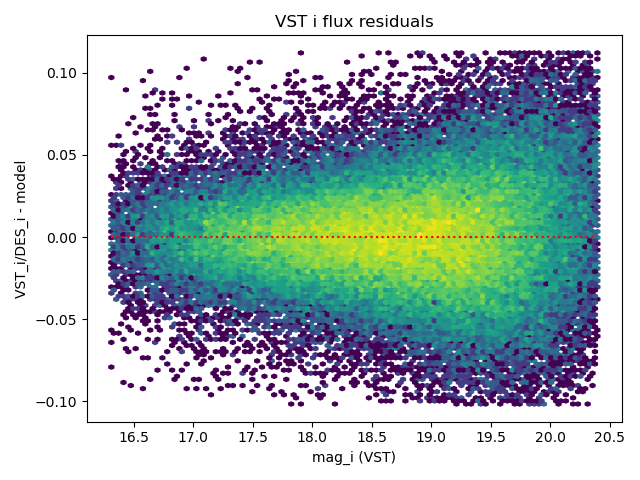
\includegraphics[width=0.49\linewidth]{./figures/color_terms/VST_to_DES_band_i_flux_residuals.png}
    \caption{Same as figure (\ref{fig:acolor-vst-g}) but for \textit{i}-band.}
\end{figure}
% vst-DES z
\begin{figure}
    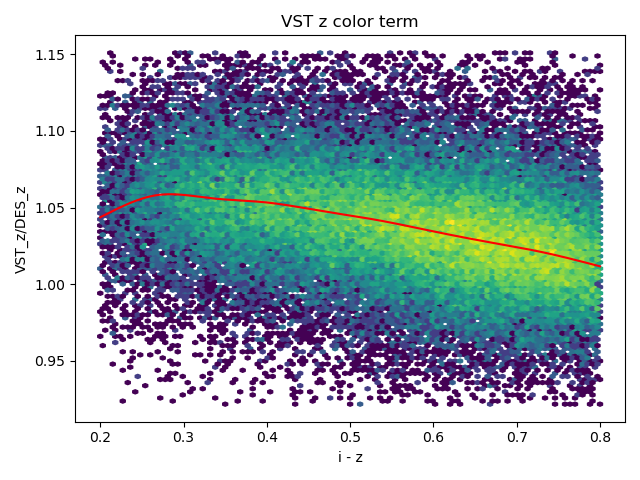
\includegraphics[width=0.49\linewidth]{./figures/color_terms/VST_to_DES_band_z_color_term.png}
    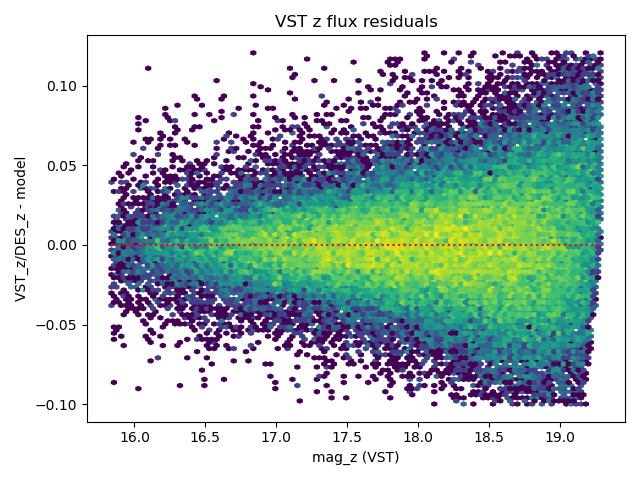
\includegraphics[width=0.49\linewidth]{./figures/color_terms/VST_to_DES_band_z_flux_residuals.png}
    \caption{Same as figure (\ref{fig:acolor-vst-g}) but for \textit{z}-band. Note the color transfomation is a function of i-z}
\end{figure}

\subsection{SDSS}